\documentclass[a4paper,10pt]{article}
\usepackage[italian]{babel} 
\usepackage[T1]{fontenc} 
\usepackage[utf8]{inputenc} 
\usepackage{amsfonts}
\usepackage{amsthm}
\usepackage[margin=25mm]{geometry}
\usepackage{mathtools}
\usepackage{listings}
\usepackage{centernot}
\usepackage{multicol}
\usepackage{pgfplots}
\usepackage{soul}
\usepackage{stmaryrd}
\usepackage{graphicx}

%opening
\title{Giorno 8}
\author{Lorenzo Pace}

\theoremstyle{definition}
\newtheorem{deff}{Def.}[section]
\newtheorem{lemma}[deff]{Lemma}
\newtheorem{es}[deff]{Es.}
\newtheorem{ex}[deff]{Esercizio}
\newtheorem{teo}[deff]{Teorema}
\newtheorem{prop}[deff]{Proposizione}
\lstset
{ %Formatting for code in appendix
    language=Pascal,
    otherkeywords={print, ref, nil, return, elif}, 
    basicstyle=\footnotesize,
    numbers=left,
    stepnumber=1,
    showstringspaces=false,
    tabsize=1,
    breaklines=true,
    breakatwhitespace=false,
}
\renewcommand{\qedsymbol}{\rule{1ex}{1ex}}
\setlength{\parindent}{0em}
\usetikzlibrary{shapes}
\usetikzlibrary{shapes.misc}

\newcommand{\reals}{\mathbb{R}}
\newcommand{\rationals}{\mathbb{Q}}
\newcommand{\integers}{\mathbb{Z}}
\newcommand{\naturals}{\mathbb{N}}

\tikzset{cross/.style={cross out, draw=black, minimum size=2*(#1-\pgflinewidth), inner sep=0pt, outer sep=0pt},
%default radius will be 1pt. 
cross/.default={1pt}}


\begin{document}

\begin{center}
    \LARGE Giorno 8
\end{center}
\section{Cammini minimi da sorgente unica}

Sia $G = (V, E)$ un grafo, e sia $w:E \to \reals$ una funzione che associa ad ogni arco un \emph{peso}. Un grafo associato ad una funzione peso si dice \emph{pesato}.
\begin{deff}
    Il \emph{peso di un cammino} è la somma dei pesi degli archi che lo compongono.
\end{deff}
\begin{deff}
    Il cammino di peso minimo tra due nodi di un grafo pesato si dice \emph{cammino minimo}
\end{deff}
\begin{deff}
   La distanza tra due nodi $\delta(u, v)$ è il peso del cammino minio tra i due nodi.
\end{deff}


In questa sezione analizziamo il problema di individuare i cammini minimi tra un nodo $s$ che chiamiamo \emph{sorgente} e tutti gli altri nodi del grafo. Alcuni problemi simili possono essere ricondotti a questo e risolti utilizzando gli stessi metodi:
\begin{enumerate}
 \item \textbf{Cammini minimi a destinazione unica}: Si invertono le direzioni degli archi, si tratta la destinazione come sorgente;
 \item \textbf{Cammini minimi tra una coppia di nodi}: Sia uno dei due nodi la sorgente, il problema è risolto da un algoritmo che trova i cammini minimi da sorgente unica.
 \item \textbf{Cammini minimi tra tutte le coppie di nodi}: Può essere risolto iterando un algoritmo che trova i cammini minimi da sorgente unica, ma esiste una soluzione migliore.
\end{enumerate}
\subsection{Algoritmo di Dijkstra}
Ad ogni nodo $v$ sono associati due campi: 
\begin{itemize}
 \item $v.d$, stima per eccesso del peso del cammino tra $s$ e $v$: \hspace{2mm} $v.d \geq \delta(s, v)$
 \item $v.p$, alla fine dell'esecuzione è il precedente di $v$ nel cammino tra $s$ e $v$.
\end{itemize}
\begin{enumerate}
 \item Inizialmente tutti i nodi tranne la sorgente hanno $v.p =$ nil, $v.d = \infty$, mentre $s.d = 0$.

\item Si inseriscono tutti i nodi in una coda di min-priorità con priorità $v.d$.

\item Si estrae ripetutamente, finché la CDP non è vuota, il nodo $v$ la cui stima è minima, che alla prima iterazione sarà la sorgente, e per ogni elemento $u$ di $Adj[v]$, se $u.d > v.d + w(v, u)$:
\begin{enumerate}
 \item Si pone $u.d = v.d + w(v, u)$;
 \item Si pone $u.p = v$;
 \item Si diminuisce, nella coda di priorità, il valore della chiave di $u$, ponendola $=v.d + w(v, u)$ 
\end{enumerate}
Queste tre operazioni sono dette ``di rilassamento''.

\end{enumerate}
\subsection{Complessità}
\begin{multicols}{2}
 \begin{lstlisting}[escapeinside={(?}{?)}]
Dijkstra(g, s, w):
    PQ = new min-priority queue
    s.d = 0;
    for(v (?$\in$?) g.V):
        v.d = (?$\infty$?)
        v.p = nil;
        insert(PQ, v);
    while(PQ (?$\neq \emptyset$?)):
        v = extractMin(PQ);
        for(u (?$\in$?) Adj[v]):
            if(u.d > v.d + w(v, u)):
                u.d = v.d + w(v, u);
                decreaseKey(PQ, u, v.d + w(v, u))
    
    
 \end{lstlisting}
L'algoritmo esegue $\Theta(|V|)\cdot T(insert)$ operazioni di inizializzazione, e il while costa $\Theta(|E|)\cdot (T(extractMin) + T(decreaseKey))$.

Assumendo di usare un min-heap come coda di priorità:

\begin{enumerate}
 \item costruire un Min-Heap costa $O(|V|)$
 \item extractMin costa $O(\log |V|)$
 \item decreseKey costa $O(\log |V|)$ (+ tempo ricerca, ma teniamo riferimenti tra pos heap e nodi)
\end{enumerate}
Quindi il costo totale è $O(\log |V| \cdot(|V| + |E|))$
\end{multicols}


\newpage

\subsubsection{Correttezza dell'algoritmo}
\begin{teo}
Alla fine dell'esecuzione si ha che $\forall v \in V : v.d = \delta(s, v)$ 
\end{teo}
\begin{proof}\begin{itemize}\item[]
             \end{itemize}
\bigskip
($\star$) Notiamo che per definizione $v.d \geq \delta(s, v)$;\bigskip


Sia $S$ l'insieme dei vertici estratti dalla coda. Dimostriamo per induzione sul numero di vertici in $S$.\smallskip

\emph{Hp. Ind}: Per ogni $v \in S : v.d = \delta(s, v)$.

\begin{itemize}
 \item (Base) Il primo vertice estratto è $s$, la cui distanza da $s$ è zero, ok.
 \item (Passo)
 \begin{enumerate}
  \item 
 Sia $v$ il prossimo vertice rimosso dalla coda. Sia $P$ il cammino minimo tra $s$ e $v$.
 \item Sia $(x, y)$ il primo arco di $P$ ad uscire da $S$ ($y$ potrebbe essere $v$, se il sottocammino $s \rightsquigarrow x$ fosse interamente in $S$).
 \item Dimostriamo che $y.d = \delta(s, y)$:
 
 Per ipotesi induttiva sappiamo che $x.d = \delta(s, x)$. 
 
 All'estrazione di $x$ il vertice $y$ è stato ``rilassato'', quindi: \[y.d \leq x.d + w(x, y) = \delta(s, x) w(x, y) = \delta(s, y)\]
 
 Quindi $y.d \leq \delta(s, y)$. Per $(\star)$ abbiamo $y.d \geq \delta(s, y) \implies y.d = \delta(s, y)$
 \item \[v.d \underset{(\star)}{\geq} \delta(s, v) \underset{\text{pesi non neg}}{\geq} \delta(s, y) \underset{(3)}{=} y.d \underset{\text{$v$ estr. prima di $y$}}{\geq} v.d\]
 
 Quindi abbiamo $v.d \geq \delta(s.v)\geq v.d$, quindi $v.d = \delta(s, v)$.
 \end{enumerate}

 
\end{itemize}

\end{proof}\begin{center}
                
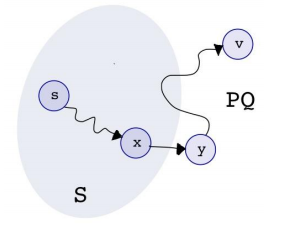
\includegraphics[scale=.7]{dim}
           \end{center}

\end{document}
